% Failure Case Gallery Appendix (10 Representative Visual Failure Cases)

This appendix presents 10 representative failure cases spanning the five archival visual breakdown categories that recur across the corpus: faded and degraded scans, historical drawings and abstract styles, crowded scenes with high object density, OCR and text--object conflicts, and occlusion with spatial overlap. Each case names the source publication (PPN) and, where relevant, its consensus entropy $H_C$, so any case can be located in the archive and re-inspected.

\section{Visual Failure Case Gallery}

\begin{figure}[!htbp]
    \centering
    \begin{subfigure}{0.40\textwidth}
        \centering
        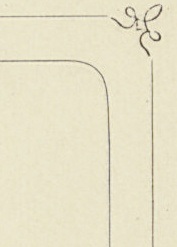
\includegraphics[width=\textwidth]{latex_assets/failure_degraded_1.jpg}
        \caption{\textbf{Case DEGRADED-1}: Blurry scan (\texttt{PPN183128149X}). $H_C=0.5000$. YOLO misses boxes; VLM infers layout.}
    \end{subfigure}
    \hfill
    \begin{subfigure}{0.40\textwidth}
        \centering
        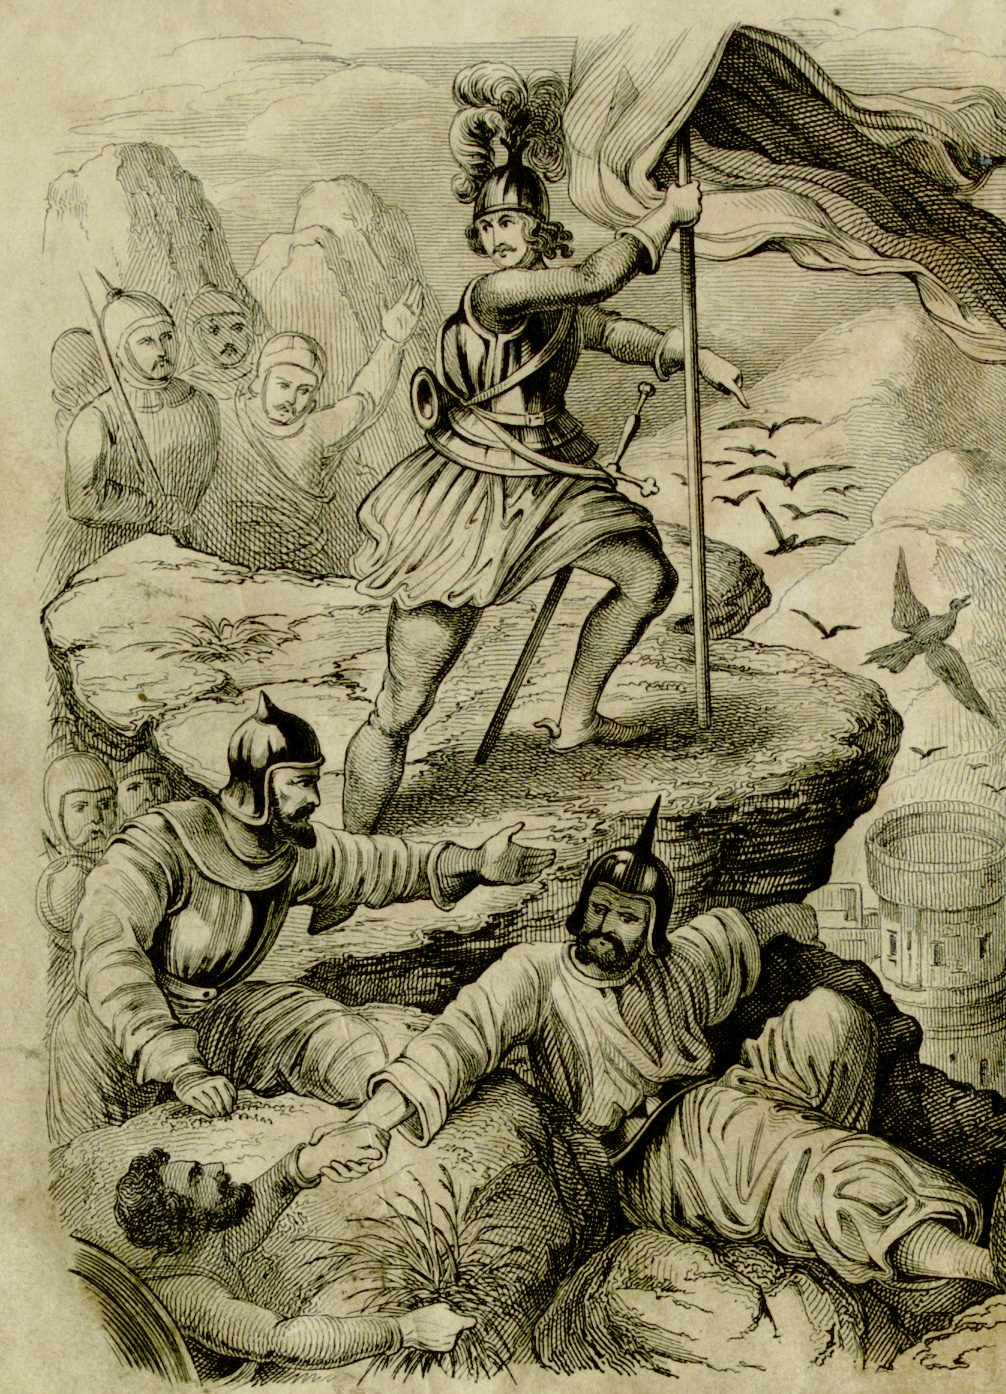
\includegraphics[width=\textwidth]{latex_assets/failure_degraded_2.jpg}
        \caption{\textbf{Case DEGRADED-2}: Blurry illustration (\texttt{PPN1802793658}). $H_C=0.4570$. YOLO box shift; VLM overconfidence.}
    \end{subfigure}

    \vspace{2mm}

    \begin{subfigure}{0.40\textwidth}
        \centering
        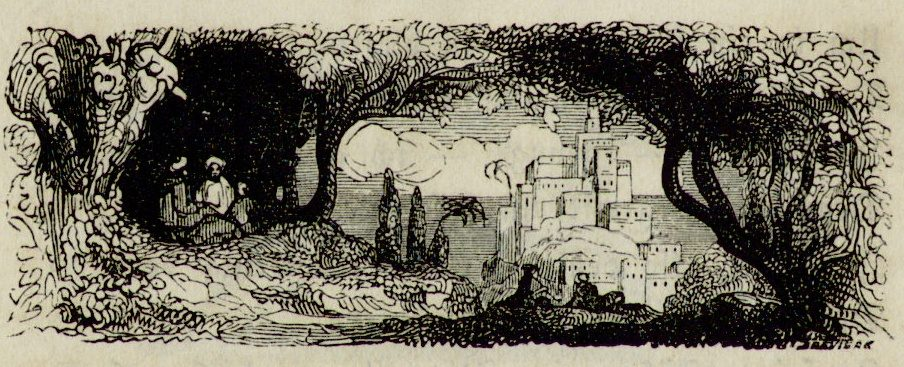
\includegraphics[width=\textwidth]{latex_assets/failure_drawing_1.jpg}
        \caption{\textbf{Case DRAWING-1}: Hand sketch (\texttt{PPN1816431109}). $H_C=0.4570$. Abstract linework causes YOLO proposal failure.}
    \end{subfigure}
    \hfill
    \begin{subfigure}{0.40\textwidth}
        \centering
        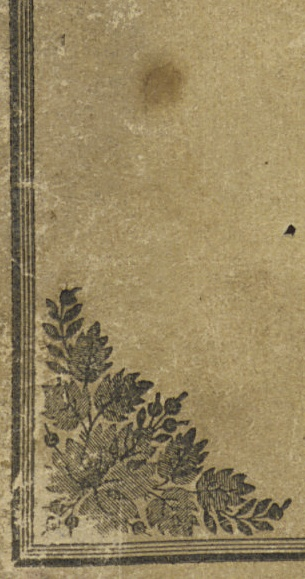
\includegraphics[width=\textwidth]{latex_assets/failure_drawing_2.jpg}
        \caption{\textbf{Case DRAWING-2}: Stylized artwork (\texttt{PPN1807545539}). $H_C=0.4488$. Hatching triggers false person detections.}
    \end{subfigure}
    \caption{Categories 1--2: faded or degraded scans (top) and historical drawings or abstract styles (bottom).}
    \label{fig:failure_cat12}
\end{figure}

\begin{figure}[!htbp]
    \centering
    \begin{subfigure}{0.40\textwidth}
        \centering
        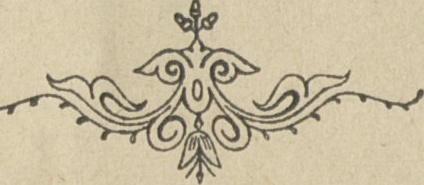
\includegraphics[width=\textwidth]{latex_assets/failure_crowded_1.jpg}
        \caption{\textbf{Case CROWDED-1}: High density ($n=9$, \texttt{PPN175936214X}). $H_C=0.5000$. Bounding box overlap merge conflicts.}
    \end{subfigure}
    \hfill
    \begin{subfigure}{0.40\textwidth}
        \centering
        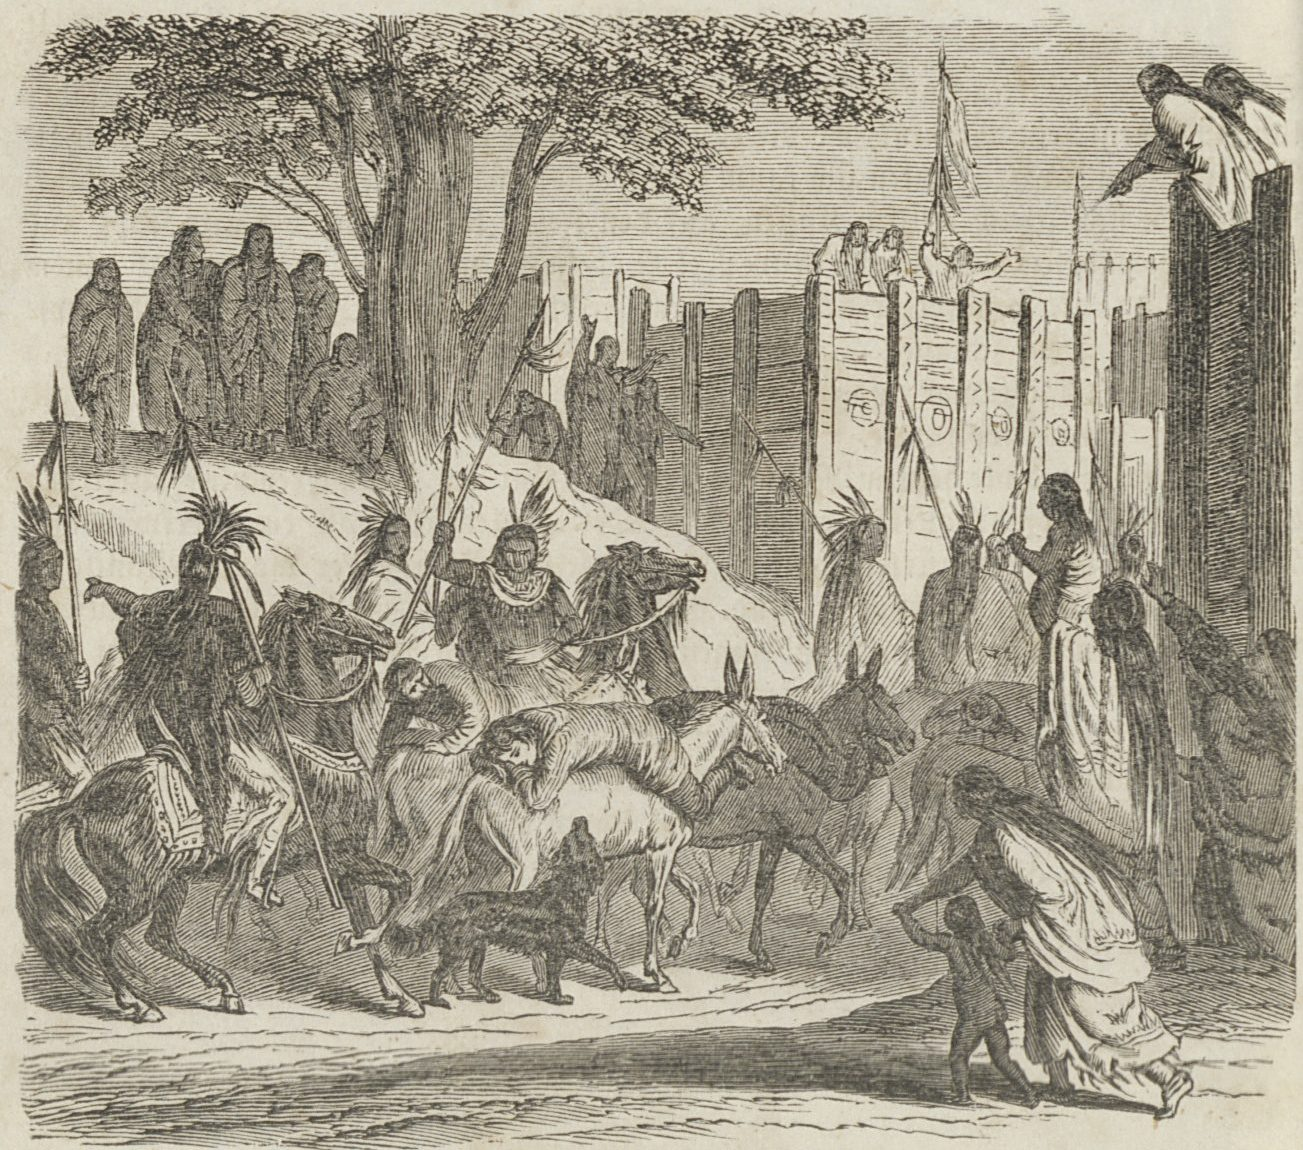
\includegraphics[width=\textwidth]{latex_assets/failure_crowded_2.jpg}
        \caption{\textbf{Case CROWDED-2}: Dense scene ($n=12$, \texttt{PPN1837132763}). $H_C=0.4685$. Visual clutter suppresses NMS proposals.}
    \end{subfigure}

    \vspace{2mm}

    \begin{subfigure}{0.40\textwidth}
        \centering
        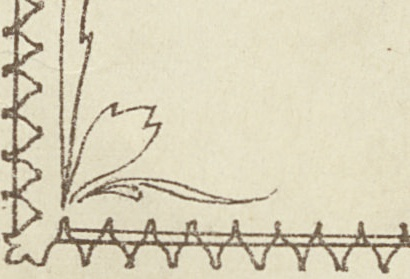
\includegraphics[width=\textwidth]{latex_assets/failure_text_conflict_1.jpg}
        \caption{\textbf{Case TEXT-1}: Printed text page (\texttt{PPN1837925887}). $H_C=0.5000$. OCR text density conflicts with VLM caption.}
    \end{subfigure}
    \hfill
    \begin{subfigure}{0.40\textwidth}
        \centering
        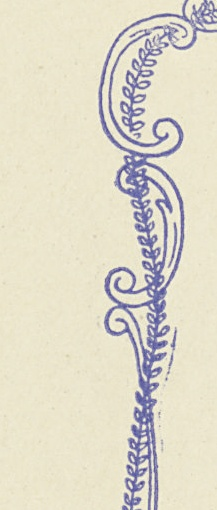
\includegraphics[width=\textwidth]{latex_assets/failure_text_conflict_2.jpg}
        \caption{\textbf{Case TEXT-2}: Margin notes (\texttt{PPN1859200435}). $H_C=0.5000$. Layout typography disrupts cross-modal consensus.}
    \end{subfigure}
    \caption{Categories 3--4: crowded scenes with high object density (top) and OCR/text--object conflicts (bottom).}
    \label{fig:failure_cat34}
\end{figure}

\begin{figure}[!htbp]
    \centering
    \begin{subfigure}{0.40\textwidth}
        \centering
        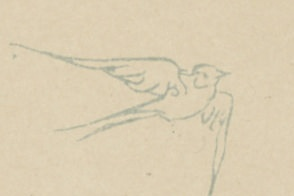
\includegraphics[width=\textwidth]{latex_assets/failure_occlusion_1.jpg}
        \caption{\textbf{Case OCCLUSION-1}: Partial occlusion (\texttt{PPN176263855X}). $H_C=0.4135$. Overlapping boundaries reject box proposals.}
    \end{subfigure}
    \hfill
    \begin{subfigure}{0.40\textwidth}
        \centering
        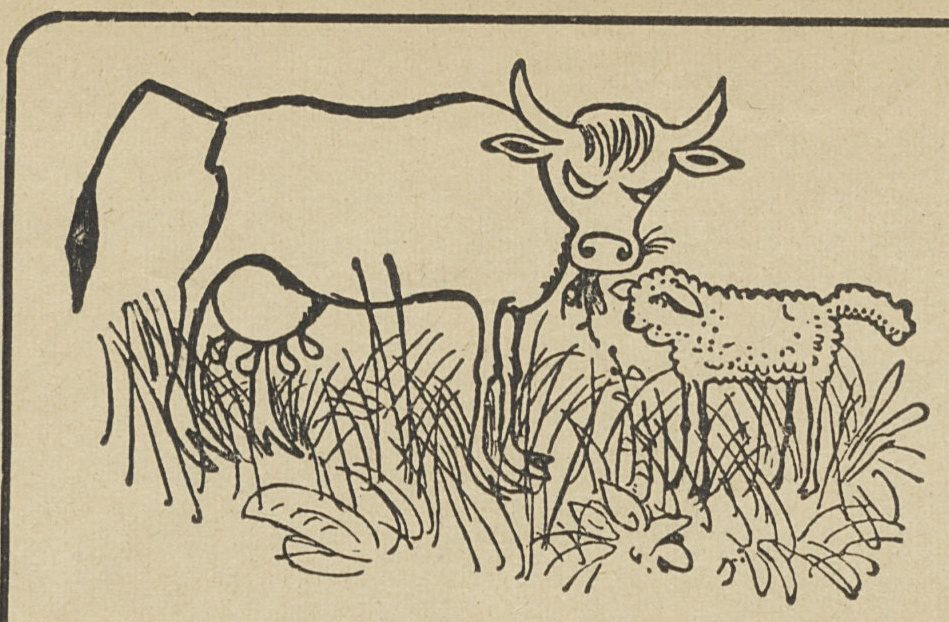
\includegraphics[width=\textwidth]{latex_assets/failure_occlusion_2.jpg}
        \caption{\textbf{Case OCCLUSION-2}: Overlapping figures (\texttt{PPN1859148263}). $H_C=0.4135$. VLM merges two subjects into one entity.}
    \end{subfigure}
    \caption{Category 5: occlusion and spatial overlap failures.}
    \label{fig:failure_cat5}
\end{figure}
